\documentclass[12pt,a4paper]{article}

% Encoding (must be before other packages)
\usepackage[utf8]{inputenc}
\usepackage[T1]{fontenc}

% Layout
\usepackage[margin=2.5cm, headheight=15pt]{geometry}
\usepackage{graphicx}
\usepackage{booktabs}
\usepackage{longtable}
\usepackage{tabularx}
\usepackage{array}
\usepackage{xcolor}
\usepackage{hyperref}
\usepackage{enumitem}
\usepackage{titlesec}
\usepackage{fancyhdr}
\usepackage{parskip}
\usepackage[protrusion=true,expansion=false]{microtype}
\usepackage{listings}
\usepackage{caption}
\usepackage{amsmath,amssymb}
\usepackage{ragged2e}

% Colors
\definecolor{iiitbblue}{RGB}{0,62,126}
\definecolor{lightgray}{RGB}{245,245,245}
\definecolor{darkgray}{RGB}{80,80,80}
\definecolor{codegreen}{rgb}{0,0.6,0}
\definecolor{codepurple}{rgb}{0.58,0,0.82}

% Hyperref — no colored text, no visible borders, no anchor dots
\hypersetup{
    colorlinks=false,
    pdfborder={0 0 0},
    pdftitle={Neurosymbolic Sudoku Solver -- AID 851},
    pdfauthor={Shikhar (MT2025114)}
}

% Section formatting
\titleformat{\section}{\large\bfseries\color{iiitbblue}}{\thesection.}{0.6em}{}[\titlerule]
\titleformat{\subsection}{\normalsize\bfseries\color{darkgray}}{\thesubsection}{0.6em}{}
\titleformat{\subsubsection}{\normalsize\itshape}{\thesubsubsection}{0.6em}{}

% Header / Footer
\pagestyle{fancy}
\fancyhf{}
\lhead{\small\color{darkgray} AID 851 Machine Reasoning -- Neurosymbolic Sudoku}
\rhead{\small\color{darkgray} Shikhar | MT2025114}
\cfoot{\thepage}
\renewcommand{\headrulewidth}{0.4pt}

% Listings style
\lstset{
  backgroundcolor=\color{lightgray},
  basicstyle=\ttfamily\small,
  keywordstyle=\color{iiitbblue}\bfseries,
  commentstyle=\color{codegreen},
  stringstyle=\color{codepurple},
  breaklines=true,
  frame=single,
  rulecolor=\color{darkgray},
  captionpos=b
}

% Column types
\newcolumntype{L}[1]{>{\RaggedRight\arraybackslash}p{#1}}
\newcolumntype{C}[1]{>{\Centering\arraybackslash}p{#1}}

%==============================================================================
\begin{document}
\begin{titlepage}
\begin{center}
\vspace*{1.5cm}
{\large\bfseries International Institute of Information Technology Bangalore}\\[0.5em]
{\normalsize AID 851 -- Machine Reasoning}\\[0.2em]
{\small M.Tech 2025\,--\,2027 \textbar\ Semester III}\\[1.5em]
{\color{darkgray}\rule{\linewidth}{0.6pt}}\\[2.5em]
{\LARGE\bfseries Neurosymbolic Sudoku Solver}\\[0.7em]
{\large\itshape Diagonal Sudoku: a neural network proposes, a CDCL SAT solver verifies and repairs}\\[2em]
{\color{darkgray}\rule{0.44\linewidth}{0.4pt}}\enspace{\color{iiitbblue}$\bullet$}\enspace{\color{darkgray}\rule{0.44\linewidth}{0.4pt}}\\[3em]
{\normalsize\bfseries Shikhar (MT2025114)}\\[1.2em]
{\normalsize Project Report -- 18 November 2026}\\
\vfill

\includegraphics[width=4cm]{IIITB_logo.png}
\vspace{3cm}
\end{center}
\end{titlepage}
\pagenumbering{roman}
\tableofcontents
\newpage
\pagenumbering{arabic}

\section{Abstract}
I built a solver for \textbf{Diagonal Sudoku} (X-Sudoku: besides rows, columns and $3\times3$ boxes, both main
diagonals must contain each digit $1$--$9$ exactly once) that combines a \textbf{neural} module with a
\textbf{symbolic} one. The symbolic module is a CDCL SAT solver written from scratch (two-watched-literal propagation,
first-UIP learning, VSIDS, restarts, assumptions and UNSAT cores) working on a CNF encoding of the rules. The neural module
is an MLP that reads a puzzle together with symbolic candidate masks and predicts a probability for every digit in every empty cell.
The two are coupled in two ways: (i) the probabilities \emph{guide} the SAT search (initial branching order and polarity), and
(ii) the most confident predictions are passed to the solver as \emph{hints} (assumptions); if hints contradict the rules, the solver
returns an \emph{UNSAT core}, the offending hints are dropped, and search resumes (core-guided repair of the network's output).
Correctness never depends on the network: every returned solution is a model of the CNF, and uniqueness is checked symbolically.
Puzzles are read from a text file in a single strict format (\texttt{board = [[6, \_, \_, \dots], \dots]} with \texttt{\_} for blanks).
On $60$ random minimal puzzles the neural guidance reduces the worst-case number of conflicts from $158$ to $107$ and the mean from $22.5$ to $20.9$
(a modest gain, reported with its limits), while the network on its own produces \emph{no} valid grid. Compared with classical
backtracking (MRV), CDCL needs about $600\times$ fewer search steps on minimal puzzles ($13$ conflicts vs.\ $7{,}763$ nodes).

\section{Problem Statement and Goals}
The AID~851 project list suggests ``Sudoku solver -- use neurosymbolic reasoning''. This stand-alone (individual) project uses the \textbf{diagonal (X) variant}, which adds two constraints
to standard Sudoku (the classic rules are available with a flag). Goals:
\begin{enumerate}[nosep]
  \item Implement the symbolic engine ourselves: propositional encoding + CDCL with learning, VSIDS, restarts, assumptions and unsat cores.
  \item Add a neural component and a principled neural--symbolic interface whose output is always \emph{verified} by logic.
  \item Take puzzles from a plain text file in one strict, human-friendly format.
  \item Evaluate against baselines (CSP backtracking, plain CDCL, neural-only) with ablations, reporting negative results honestly.
\end{enumerate}
\textbf{Constraints.} No GPU or deep-learning framework was available, so the network is a scikit-learn MLP; training data are generated by my own
puzzle generator (random puzzles with unique solutions); the neural net is small, so its predictions are weak on hard puzzles.

\section{System Architecture}
\begin{center}\small
\fbox{\texttt{board = [[...]]} text file} $\rightarrow$ \fbox{strict parser (81 cells)}\\[4pt]
$\Downarrow$\\[4pt]
\fbox{symbolic candidate masks} $\rightarrow$ \fbox{\textbf{neural}: MLP $\Rightarrow P\in\mathbb{R}^{81\times9}$}\\[4pt]
$\Downarrow$ \quad (guidance + hints)\\[4pt]
\fbox{\textbf{symbolic}: CNF + CDCL under assumptions} $\leftrightarrow$ \fbox{core-guided hint repair}\\[4pt]
$\Downarrow$\\[4pt]
\fbox{verified solution + uniqueness check}
\end{center}

\begin{table}[h]\centering\small
\begin{tabular}{@{}L{5.2cm}L{9.5cm}@{}}\toprule
Module & Responsibility\\\midrule
\texttt{sudoku\_ns/sat.py} & CDCL solver: 2-watched literals, 1-UIP learning, VSIDS, Luby restarts, assumptions, cores, guidance hook\\
\texttt{sudoku\_ns/encoding.py}, \texttt{config.py} & CNF encoding (729 variables); rule variant (diagonal / standard)\\
\texttt{sudoku\_ns/csp.py} & Baseline bit-mask MRV backtracking; solution counting\\
\texttt{sudoku\_ns/generator.py} & Random puzzles with unique solutions; symmetries; strict input parser\\
\texttt{sudoku\_ns/neural.py} & Neural module: features, MLP, training\\
\texttt{sudoku\_ns/neurosym.py} & Neural--symbolic interface: guidance, hints, core-guided repair\\
\texttt{sudoku\_ns/explain.py} & Plain-language explanation of conflicts (unsatisfied conditions)\\
\texttt{main.py}, \texttt{tests/}, \texttt{experiments/} & CLI, unit tests, reproduction of all results\\\bottomrule
\end{tabular}
\caption{Project structure.}
\end{table}

\section{Methodology}
\subsection{Input format}
The only accepted input is a text file containing a Python-style list (lines starting with \texttt{\#} are comments):
\begin{lstlisting}
# variant: diagonal      (optional comment line: diagonal | standard)
board = [
    [6, _, _, _, 9, 8, _, _, 4],
    [_, 1, _, _, _, _, 8, _, 9],
    ...                          (9 rows of 9 entries)
]
\end{lstlisting}
Entries are digits $1$--$9$ or \texttt{\_} (blank). \texttt{0}, \texttt{.}, 81-character strings and other layouts are rejected with an error message.
\texttt{python main.py} with no arguments solves the file \texttt{standard\_classic.txt} in \texttt{examples/inputs/}; its \texttt{\# variant: standard} line selects the classic rules
(the program default is diagonal rules, and \texttt{--variant} overrides the file).

\subsection{Symbolic module: SAT encoding}
Variable $x_{r,c,d}$ is true iff cell $(r,c)$ holds digit $d$ ($729$ variables, DIMACS id $81r+9c+d$).
Clauses: (i) every cell has at least one digit, (ii) at most one digit per cell,
(iii) for each of the 29 units (9 rows, 9 columns, 9 boxes and the 2 diagonals) and digit $d$: $d$ occurs at most once, and
(iv) \emph{redundant} clauses stating $d$ occurs at least once in the unit. Clues are not unit clauses but \emph{assumptions}, so one solver instance
can be queried repeatedly. Section~\ref{sec:solver} shows the redundant clauses (iv) cut conflicts by $10\times$. Diagonal versus standard rules differ only in the list of units
(\texttt{sudoku\_ns/config.py}).

\subsection{CDCL solver}
The solver follows MiniSat: unit propagation with two watched literals; on a conflict, first-UIP analysis produces a learned clause and a non-chronological
backjump; VSIDS with decay, phase saving and Luby restarts. For assumptions it implements \texttt{analyzeFinal}: if the assumptions are contradictory it returns the
subset responsible, the \emph{UNSAT core}. Uniqueness of the solution is tested with a selector literal $s$ and a blocking clause $(\neg s\vee\bigvee_{x\in M}\neg x)$
over the true variables $M$ of the found model; UNSAT under $s$ means the solution is unique. A method \texttt{set\_guidance} lets an external model set initial polarities and VSIDS activities.

\subsection{Neural module}
\textbf{Features.} For a puzzle: the one-hot encoding of the $81$ cells ($81\times10$) \emph{and} the symbolic candidate mask ($81\times9$: digits not yet used by any peer in the row,
column, box or diagonals), so symbolic elimination is itself an input of the network.
\textbf{Model.} MLP regressor with two hidden layers of $768$ units predicting a one-hot of the solution ($81\times9$); outputs are clipped, multiplied by the candidate mask and normalised per cell,
giving $P_{i,d}$.
\textbf{Training data.} $1500$ random diagonal puzzles with unique solutions ($22$--$34$ clues), each expanded with $16$ diagonal-preserving symmetries
(digit relabelling, rotations, mirror): $24{,}000$ samples. Test puzzles are drawn from different seeds.

\subsection{Neural--symbolic interface}
The network is treated as an unreliable \emph{proposer}. Four solver modes are compared:
\begin{description}[nosep]
  \item[plain] CDCL alone (baseline).
  \item[guided] $P$ sets CDCL's initial branching: activity of $x_{i,d}$ is $P_{i,d}$ and its polarity is true for the arg-max digit of each cell.
  \item[hints] The cells whose top prediction has confidence $\ge\tau$ ($\tau=0.9$) are assumed as hints. If the solver answers UNSAT, the core contains the hints that
        cannot all hold together with the givens; those hints are \textbf{dropped} and the solver is called again (core-guided repair). When no hint remains in the core, the
        givens themselves are contradictory and UNSAT is reported.
  \item[both] hints and guidance.
\end{description}
Soundness: a model found under hints satisfies the givens and all rules, hence it \emph{is} the solution (uniqueness is checked separately); guidance only changes the search order.
The network can therefore speed the solver up but can never make an answer wrong.

\section{Experimental Results}
All numbers come from \texttt{experiments/run\_experiments.py} (fixed seeds; $60$ puzzles per set; results in \texttt{results/results.json}). ``Medium'' puzzles have $30$ clues, ``hard'' puzzles
are minimal (no clue can be removed; about $19$--$24$ clues).

\subsection{Quality of the neural proposals}
\begin{table}[h]\centering\footnotesize
\begin{tabular}{@{}lcccccc@{}}\toprule
 & Blank acc.\ & Valid grids & \multicolumn{4}{c}{precision (coverage), confidence $\ge$}\\
 & & & 0.5 & 0.7 & 0.9 & 0.95\\\midrule
Medium (30 clues) & 41.9\% & 0\% & 52\% (50\%) & 67\% (15\%) & 83\% (8\%) & 87\% (7\%)\\
Hard (minimal) & 27.7\% & 0\% & 38\% (17\%) & 51\% (3\%) & 69\% (1\%) & 77\% (0.7\%)\\\bottomrule
\end{tabular}
\caption{Top-1 accuracy on blank cells, rate of fully valid predicted grids, and precision/coverage as a function of the confidence threshold.}
\end{table}
\begin{figure}[h]\centering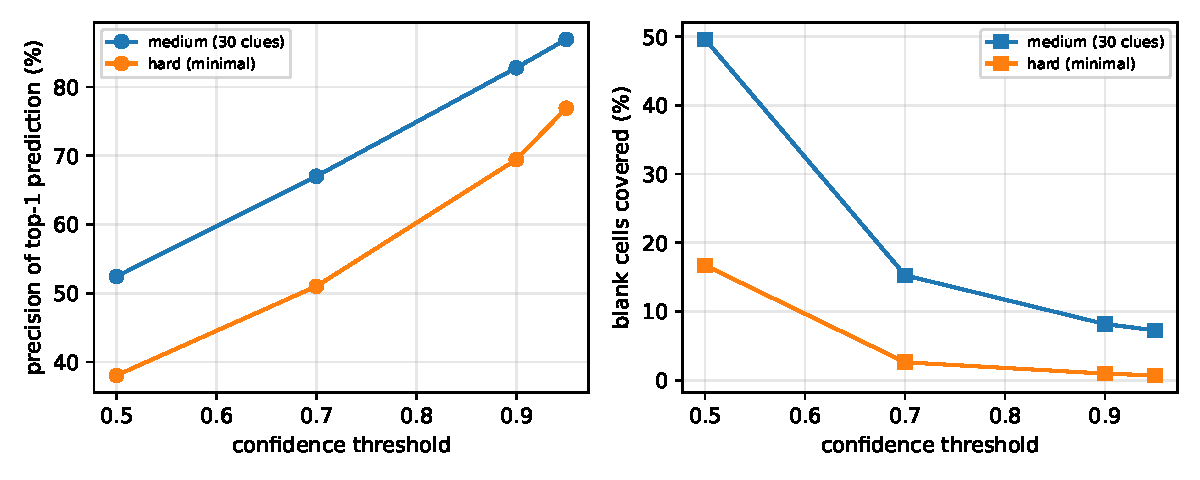
\includegraphics[width=0.85\linewidth]{figures/neural_precision.pdf}
\caption{Higher confidence means higher precision but fewer cells covered.}\end{figure}
The network alone is weak: $0\%$ of its completed grids satisfy the Sudoku rules. Its confidence is informative though (precision rises from $42\%$ to $87\%$ on medium puzzles as the threshold rises), which is what the
hint mechanism exploits. A threshold below $0.9$ yields many wrong hints.

\subsection{Effect on the SAT search}
\begin{table}[h]\centering\small
\begin{tabular}{@{}llccccc@{}}\toprule
Puzzles & Mode & decisions & conflicts (mean) & conflicts (max) & hints/dropped & time (ms)\\\midrule
Medium & plain & 0.22 & 0.083 & 2 & -- & 23.5\\
 & guided & 0.12 & 0.033 & 1 & -- & 27.5\\
 & hints & 0.08 & 0.033 & 1 & 4.2 / 0.7 & 26.0\\
 & both & 0.03 & 0.033 & 1 & 4.2 / 0.7 & 23.6\\\midrule
Hard & plain & 39.7 & 22.5 & 158 & -- & 37.5\\
 & guided & 31.7 & 20.9 & 123 & -- & 32.4\\
 & hints & 38.9 & 22.4 & 126 & 0.6 / 0.2 & 29.9\\
 & both & 30.0 & 20.9 & \textbf{107} & 0.6 / 0.2 & 32.4\\\bottomrule
\end{tabular}
\caption{Mean over $60$ puzzles per set. \emph{All} modes solved $100\%$ of puzzles correctly.}
\end{table}
\textbf{Findings.} (i) Correctness is $100\%$ in every mode, even though the network's own grids are never valid: the solver is the authority. (ii) On hard puzzles guidance reduces
mean decisions by $24\%$ ($39.7\to30.0$), the maximum conflicts from $158$ to $107$ and the mean conflicts by $7\%$; the effect on the mean conflict count is small and, with $60$ puzzles, not statistically conclusive.
(iii) The repair loop is exercised: on the medium set $0.73$ hints per puzzle were dropped after an UNSAT core, and on hard puzzles with $\tau=0.5$ about $9$ of $10$ hints are removed by repair, yet
the solver still ends on the correct solution. (iv) Lowering $\tau$ did not reduce conflicts further (mean conflicts $22.0$ at $\tau=0.5$, $23.0$ at $0.7$, $22.4$ at $0.9$), so cautious hints ($\tau=0.9$) are enough.
(v) In wall-clock time the differences are within noise, because CNF construction ($\approx20$\,ms) and the network call dominate for such small instances. The honest conclusion is that on $9\times9$ Sudoku
the CDCL solver is already so strong that a small MLP can help only marginally; the value of the design is the \emph{verified} neural--symbolic interface, which would matter more for larger or harder instances.

\subsection{Explaining unsatisfied conditions}
Running \texttt{python main.py solve-board FILE --explain} shows why the search sometimes cannot move forward. The CDCL solver
exposes a hook at every \emph{conflict}, i.e.\ whenever some clause (a Sudoku rule) is violated under the current partial assignment. The module
\texttt{sudoku\_ns/explain.py} translates it into Sudoku language: (i) the \textbf{unsatisfied condition}, e.g.\ ``cell r8c2 has no candidate digit left'', ``digit 4 has no place left in column 9'' or
``digit 5 would appear twice in the anti-diagonal''; (ii) the \textbf{chain of forced consequences} from the guesses to the conflict, each step with its reason (``r4c3 $\neq$ 3 because r7c3 = 3 is in column 3'');
(iii) the \textbf{learned rule} (the guesses that cannot all be true together) and the \textbf{backjump}. If a puzzle is solved by pure deduction (no conflict), the tool shows a ``what if'' wrong guess and the rule it violates, e.g.\ \emph{``What if r1c7 = 4? Then cell r1c8 would have to hold two digits: 1 and 9 are each forced into r1c8 because it is the only place left for them in box 3.''}
For a random minimal puzzle the first conflict is typically caused by a chain of $50$+ forced steps ending in a cell with no candidates, which illustrates why plain deduction is not enough for hard puzzles and conflict learning pays off.

\subsection{Why not neural only?}
The network's completed grids satisfy all Sudoku rules for $0\%$ of puzzles, with $42\%$/$28\%$ blank-cell accuracy (medium/hard). Learned constraint satisfaction is approximate; SAT guarantees correctness.

\subsection{Solver benchmarks and ablations}\label{sec:solver}
\begin{table}[h]\centering\small
\begin{tabular}{@{}lcccc@{}}\toprule
Mean conflicts (CDCL) / nodes (CSP) & easy (36) & medium (30) & minimal & hardest of 60\\\midrule
CDCL (VSIDS + restarts) & 0.0 & 0.0 & 13.2 & 107\\
CDCL without VSIDS & 0.0 & 0.2 & 63.2 & 173\\
CDCL without restarts & 0.0 & 0.0 & 13.2 & 106\\
CSP backtracking (MRV) & 45.0 & 61.4 & 7763 & 15598\\\bottomrule
\end{tabular}
\caption{Search effort on diagonal puzzles (40 random puzzles per class; ``hardest'' is the most conflict-heavy of 60 random minimal puzzles).}
\end{table}
\begin{figure}[h]\centering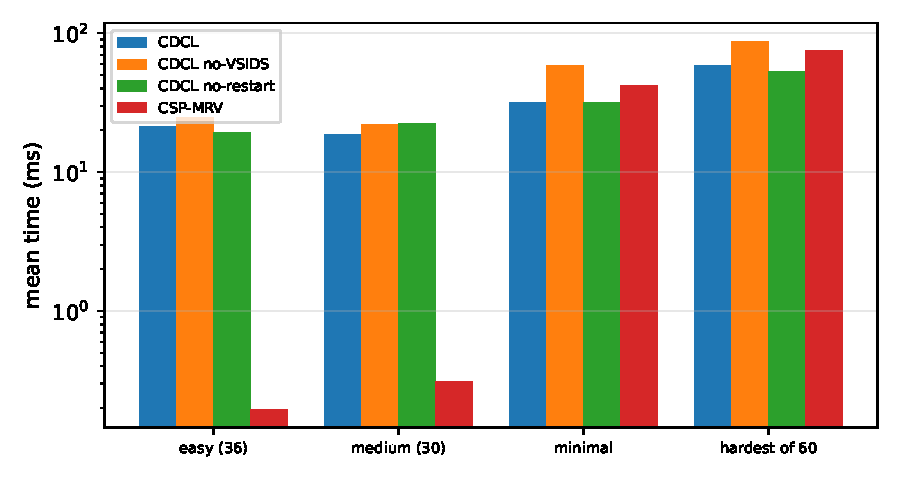
\includegraphics[width=0.7\linewidth]{figures/solver_bench.pdf}
\caption{Mean wall-clock time (log scale). CDCL times include building the CNF ($\approx20$\,ms).}\end{figure}
(i) CDCL needs orders of magnitude less search than CSP backtracking ($13$ conflicts vs.\ $7{,}763$ nodes on minimal puzzles; $107$ vs.\ $15{,}598$ on the hardest one).
(ii) VSIDS matters on hard puzzles ($13.2$ vs.\ $63.2$ conflicts); restarts make no difference at this size. (iii) The redundant ``digit occurs at least once in each unit'' clauses reduce mean conflicts from $149.6$ to $15.0$ on minimal puzzles.
(iv) In wall-clock time the pure-Python CDCL ($\approx20$\,ms, dominated by clause construction) is slower than the bit-mask CSP solver on easy puzzles ($<1$\,ms), but faster on minimal ($31$ vs.\ $42$\,ms) and hardest ($59$ vs.\ $76$\,ms) ones.

\section{Conclusions}
I built a Diagonal Sudoku solver in which a neural network proposes and a CDCL SAT solver verifies, repairs and completes. Unsat cores provide the interface: they identify which of the network's
confident guesses are mutually inconsistent with the rules, so wrong guesses are removed rather than trusted. The full pipeline is $100\%$ correct on all tested puzzles even though the network by itself never outputs a valid grid.
The neural guidance gave a measurable but modest search reduction (worst case $158\to107$ conflicts), reported here with its limits.

\textbf{Limitations.} Small MLP and synthetic training puzzles; no statistical significance testing; CNF construction dominates run-time in pure Python; the neural model was trained for diagonal puzzles, so on classic puzzles
(\texttt{--variant standard}) its proposals are less informative (still correct, as the solver decides). \textbf{Future work:} a graph or attention network over cells/units, training with SAT-derived signals
(e.g.\ predicting learned-clause activity), larger grids (e.g.\ $16\times16$), and a MaxSAT-style weighting of hints instead of dropping them.

\section{How to Run}
\begin{lstlisting}[language=bash]
pip install -r requirements.txt
python main.py                          # solves examples/inputs/standard_classic.txt
python main.py solve-board my_board.txt # board = [[6,_,_,...],...] with _ = blank
python main.py --variant diagonal solve-board my_board.txt
python main.py solve-board f.txt --explain     # show unsatisfied conditions (conflicts) and why
python main.py random --clues 30        # random puzzle (printed in the input format) and solution
python main.py solve-board f.txt --mode plain   # plain | guided | hints | both
python main.py train                    # retrain the neural module
python experiments/run_experiments.py   # reproduce all tables and figures
\end{lstlisting}

\section{Individual Contributions}
Shikhar (MT2025114): design and implementation of the symbolic engine (CNF encoding, CDCL solver), the neural module and neural--symbolic interface, the experiments, and this report.

\end{document}
